\documentclass[11pt, letterpaper]{article}
\usepackage[utf8]{inputenc}
\usepackage{amsmath, amssymb}
\usepackage{geometry}
\geometry{margin=0.75in}
\usepackage{graphicx}
\usepackage{float}
\usepackage{caption}
\usepackage{siunitx}
\usepackage{booktabs}

\title{Programming Assignment 4}
\author{by Paz Lieghton}
\date{\small Applied Probability and Statistics. Prof. Lucas Finazzi}

\begin{document}
	\maketitle
	
	\section*{Introduction}
	This report applies four classical hypothesis tests to a dataset of 219 Argentine license plates recorded by hand from around Villa Urquiza. Each entry stores the digit substring, the letter substring, and the plate format (old: \texttt{ABC 123}; new: \texttt{AB 123 CD}). Part~A tests whether digits are uniformly distributed via a chi square goodness of fit test. Part~B compares mean digit sums between formats using thr Welch $t$-test. Part~C checks whether both formats draw letters from the same distribution. Part~D tests whether consecutive letter pairs arise independently. Part~E estimates registration years and tests whether the sample is biased toward older or newer plates. All code uses NumPy, SciPy, Pandas, and Matplotlib. References and sources were key.
	
	\section{Part A: Are the Digits Uniformly Distributed?}
	
	Under $H_0$, every digit $0$--$9$ appears with equal probability $p_k = \tfrac{1}{10}$, giving expected count $E_k = n/10$. Each plate contributes three digit characters as independent observations; we test old and new formats separately. The test statistic $\chi^2 = \sum_{k=0}^{9}(O_k - E_k)^2/E_k$ follows $\chi^2(9)$ under $H_0$.
	
	\begin{figure}[H]
		\centering
		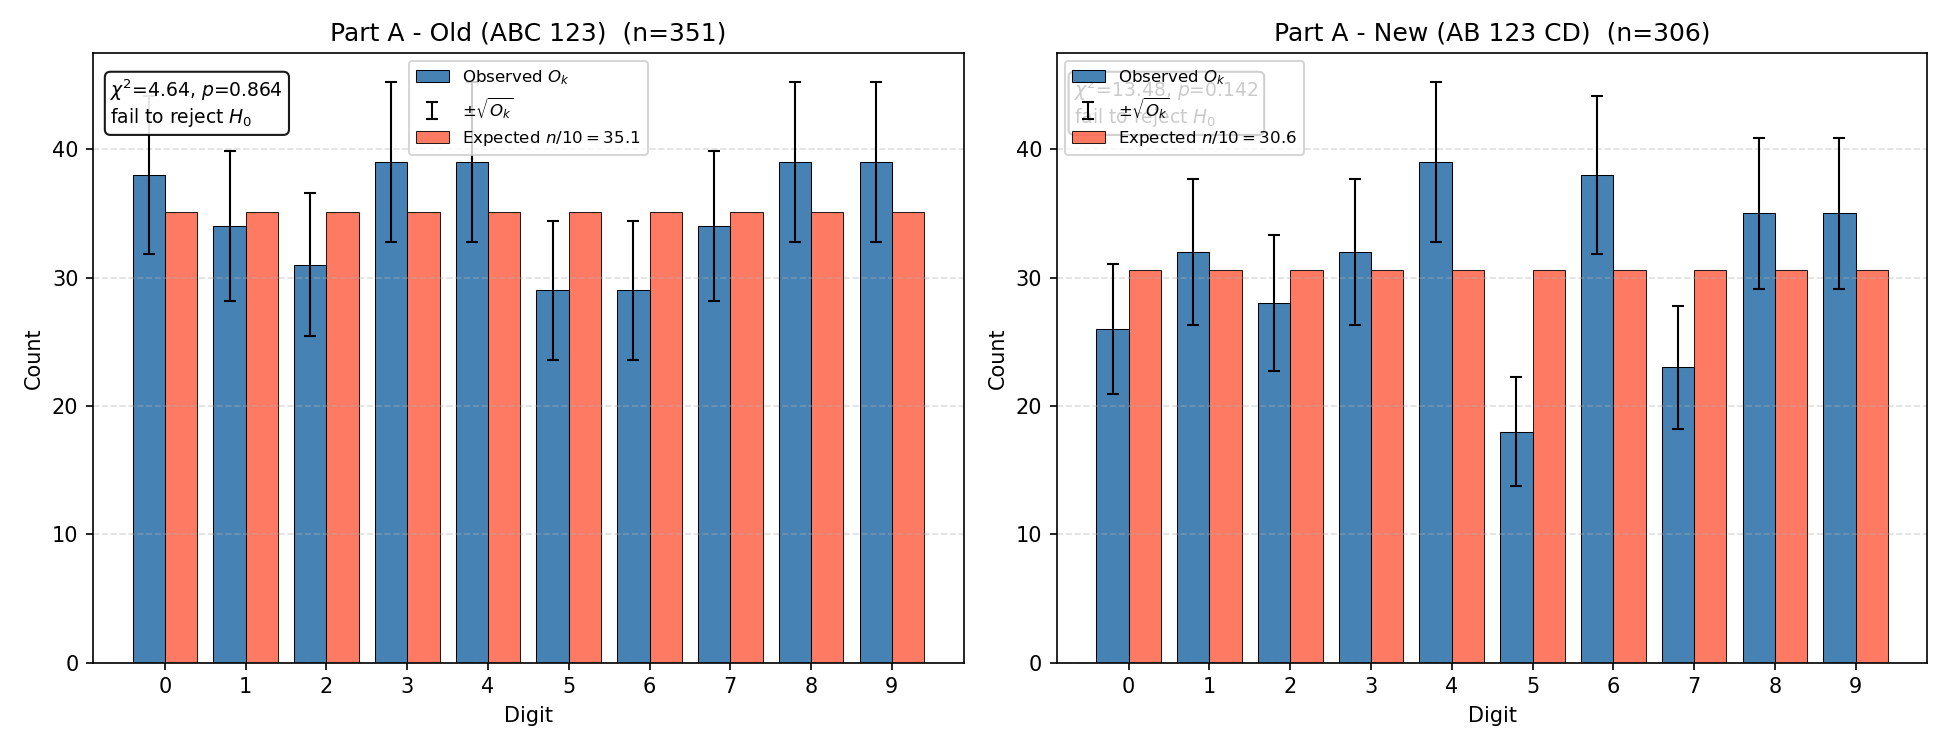
\includegraphics[width=0.90\textwidth]{fig_A2_digits.png}
		\caption{Observed digit counts $O_k$ (blue) and expected uniform counts $E_k = n/10$ (red) for old-format plates (left) and new-format plates (right). Error bars are: $\pm\sqrt{O_k}$.}
		\label{fig:A2}
	\end{figure}
	
	\begin{figure}[H]
		\centering
		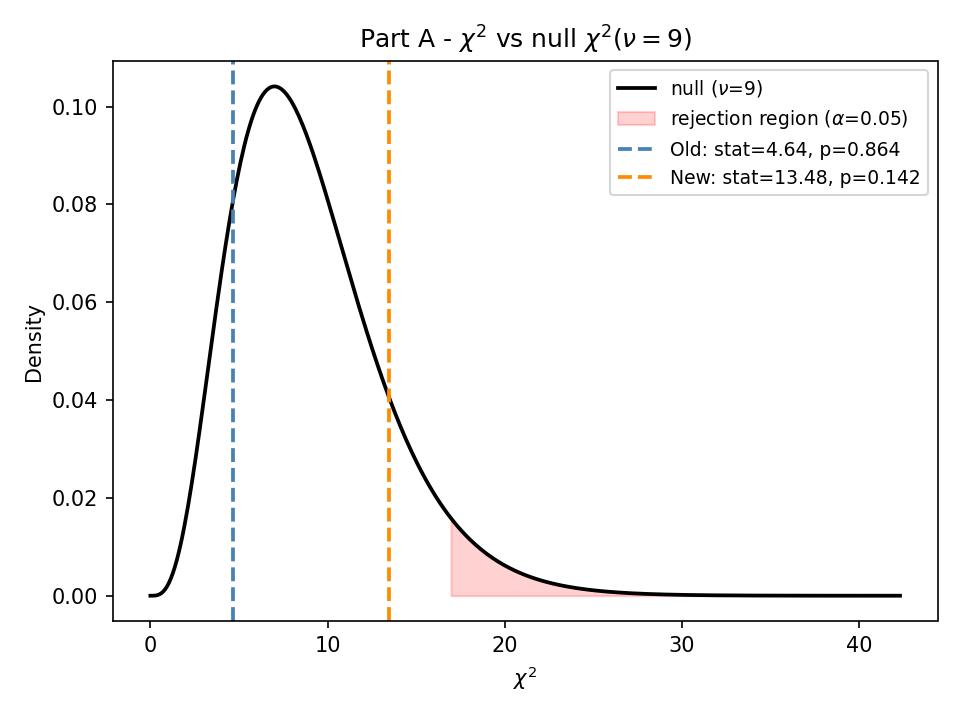
\includegraphics[width=0.60\textwidth]{fig_A3_chi2.png}
		\caption{Null $\chi^2(9)$ density with observed statistics for old (blue) and new (orange) formats. Red shaded region is the rejection tail at $\alpha = 0.05$.}
		\label{fig:A3}
	\end{figure}
	
	At $\alpha = 0.05$, both formats fail to reject $H_0$. Digit frequencies are consistent with a uniform distribution, suggesting no bias in digit assignment across either era.
	
	\section{Part B: Do Old and New Format Plates Differ in Mean Digit Sum?}
	
	The digit sum $S = d_1 + d_2 + d_3$ is approximately normal by the CLT ($\sum$ of three near-uniform variables). $H_0: \mu_{\mathrm{old}} = \mu_{\mathrm{new}}$. Normality is verified via histogram and Q-Q plot before applying Welch's $t$-test, which does not assume equal variances before testing.
	
	\begin{figure}[H]
		\centering
		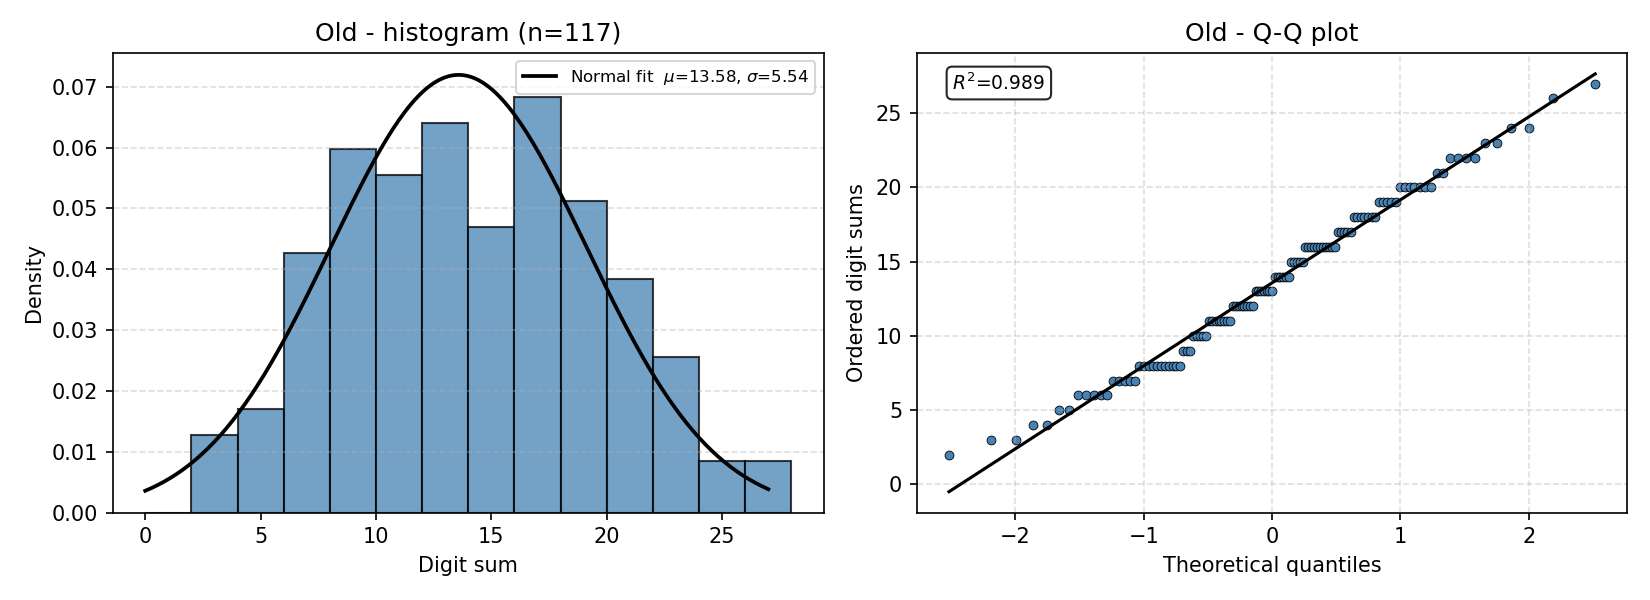
\includegraphics[width=0.85\textwidth]{fig_B1_normality_Old.png}
		\caption{Normality check for old-format digit sums: histogram with Gaussian fit (left) and Q-Q plot (right).}
	\end{figure}
	
	\begin{figure}[H]
		\centering
		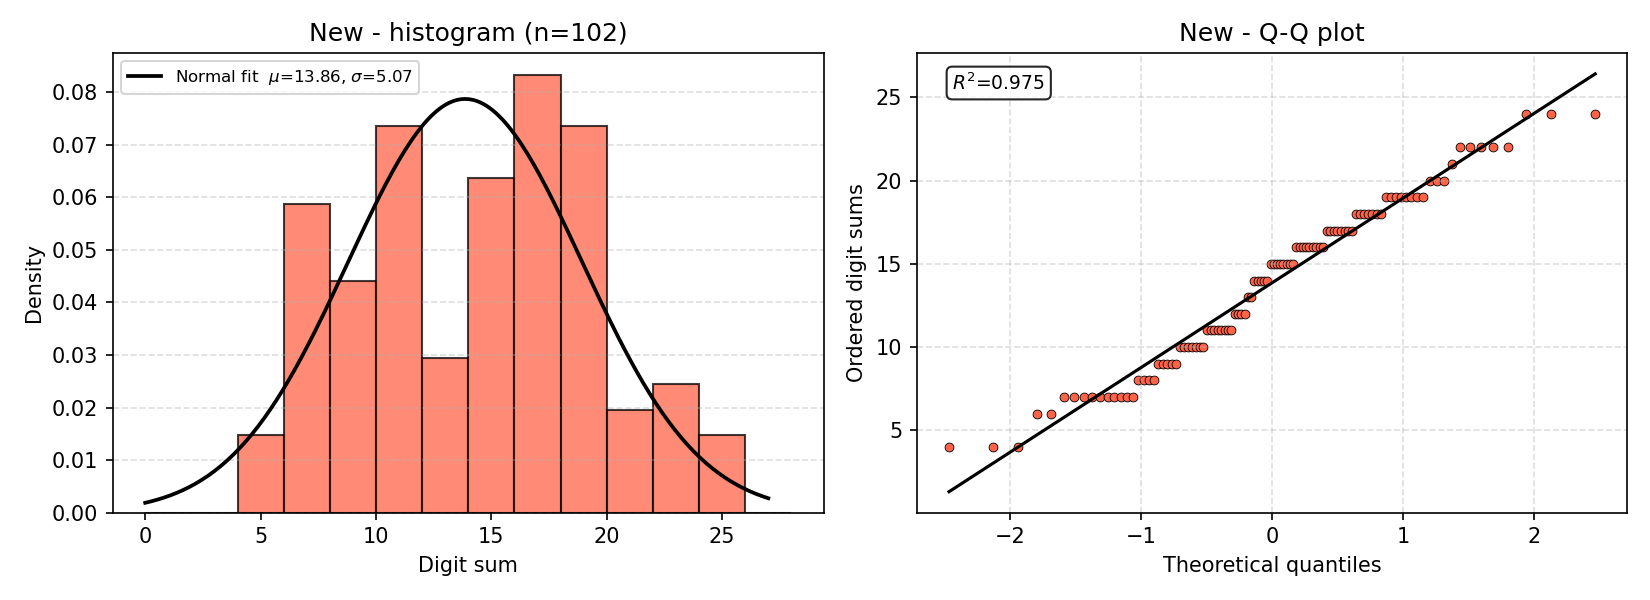
\includegraphics[width=0.85\textwidth]{fig_B1_normality_New.png}
		\caption{Normality check for new-format digit sums.}
	\end{figure}
	
	The 95\% confidence interval for $\mu_{\mathrm{old}} - \mu_{\mathrm{new}}$ is computed via the Welch--Satterthwaite effective degrees of freedom. Zero lies inside the interval, consistent with the $t$-test result: we fail to reject $H_0$. There is no significant difference in mean digit sum between the both formats (Figure~\ref{fig:B2}).
	
	\begin{figure}[H]
		\centering
		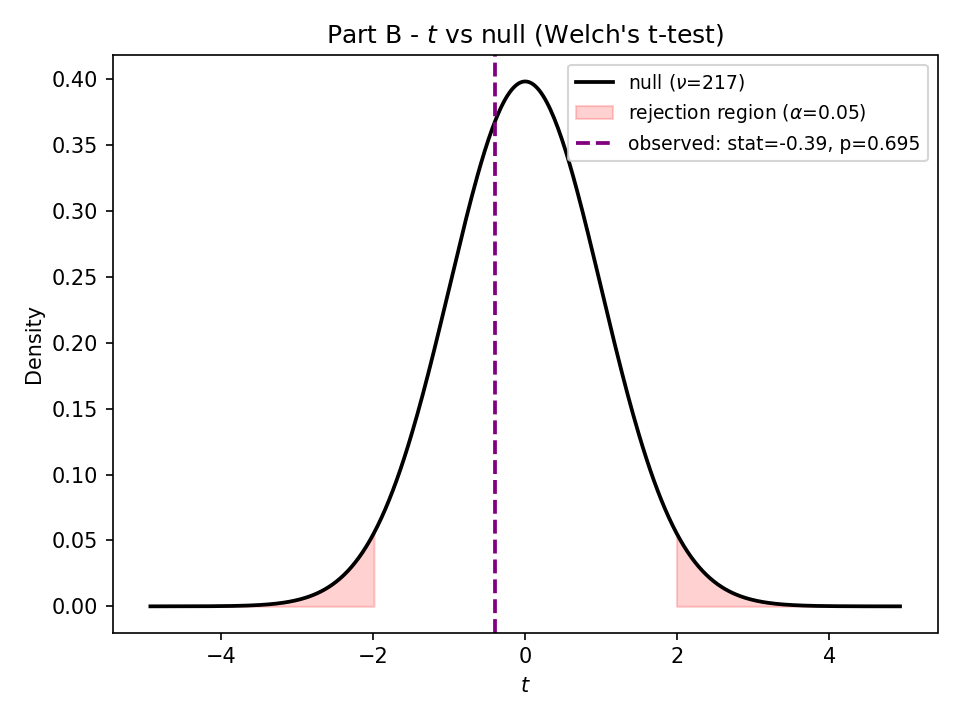
\includegraphics[width=0.60\textwidth]{fig_B2_t.png}
		\caption{Null $t(\nu)$ density (two-tailed) with the observed Welch $t$-statistic. Red shaded regions are the rejection tails at $\alpha = 0.05$.}
		\label{fig:B2}
	\end{figure}
	
	\section{Part C: Do Old and New Format Plates Draw Letters from the Same Distribution?}
	
	$H_0$: both formats draw letters from the same distribution. The new-format pool serves as the empirical reference; expected old-format counts are $E_\ell = n_{\mathrm{old}} \cdot \hat{p}_\ell^{\,\mathrm{new}}$. Bins with $E_\ell < 5$ are pooled into an ``other'' bin; letters absent from both pools (e.g.\ I, O, Q, excluded by Argentine traffic law) are dropped.
	This latter was a review done post oral as there was no research taken about characters being confused for numbers.
	
	\begin{figure}[H]
		\centering
		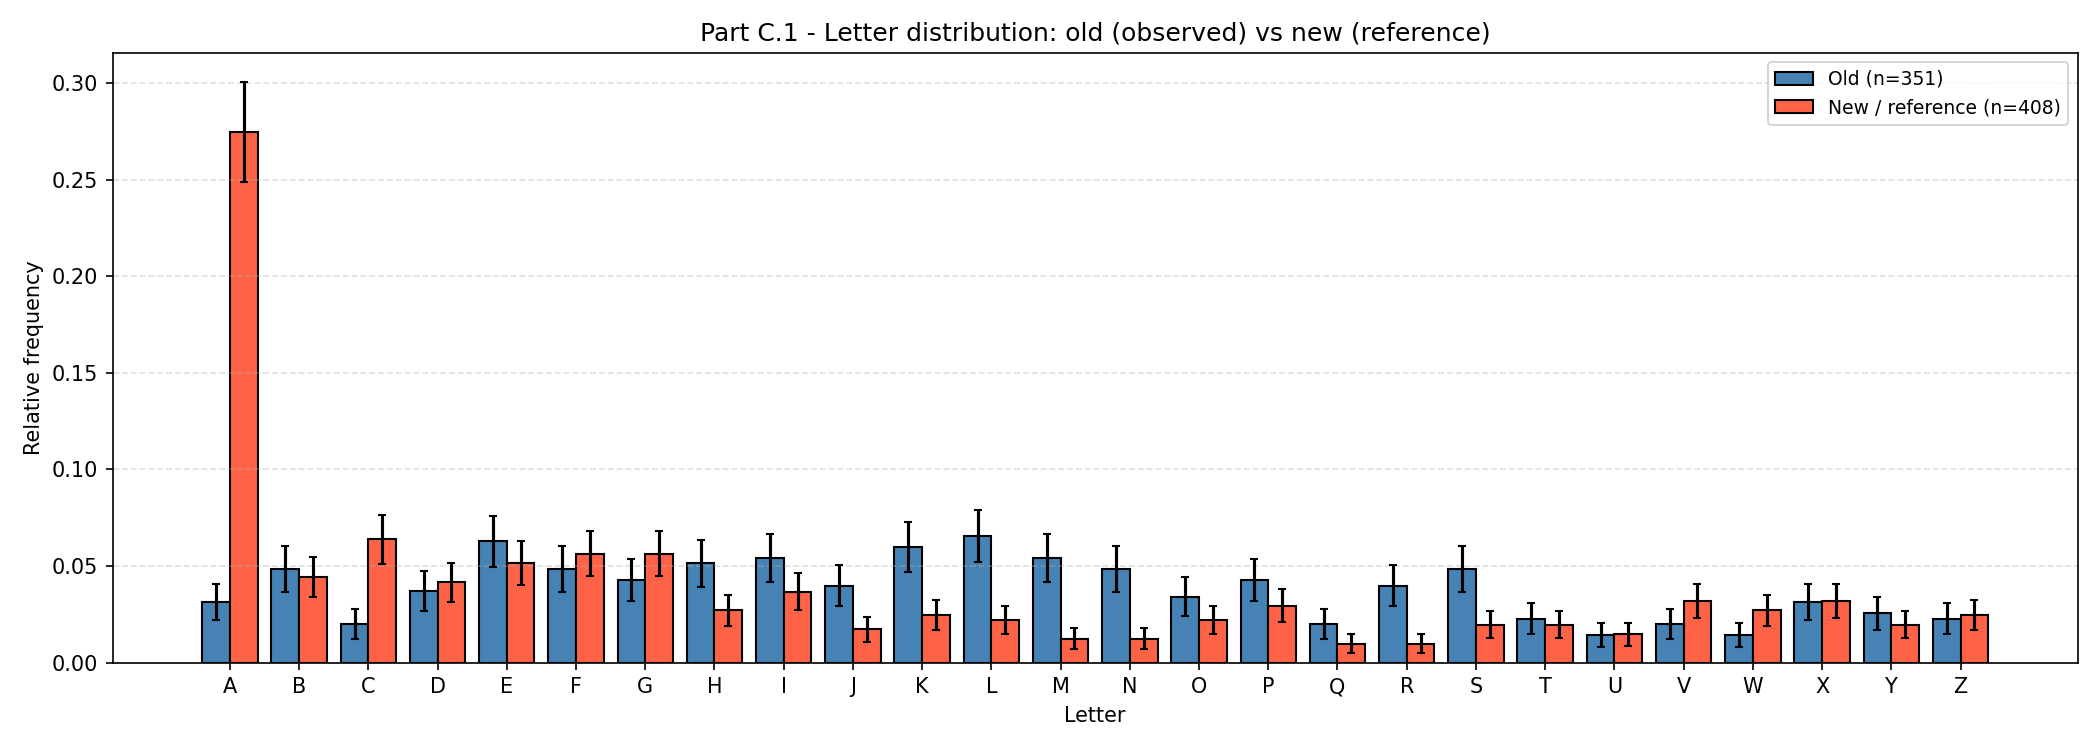
\includegraphics[width=0.90\textwidth]{fig_C1_letters.png}
		\caption{Relative letter frequencies for old-format (blue) and new-format (red) plates, with Poisson error bars $\pm\sqrt{O_\ell}/n$.}
		\label{fig:C1}
	\end{figure}
	
	\begin{figure}[H]
		\centering
		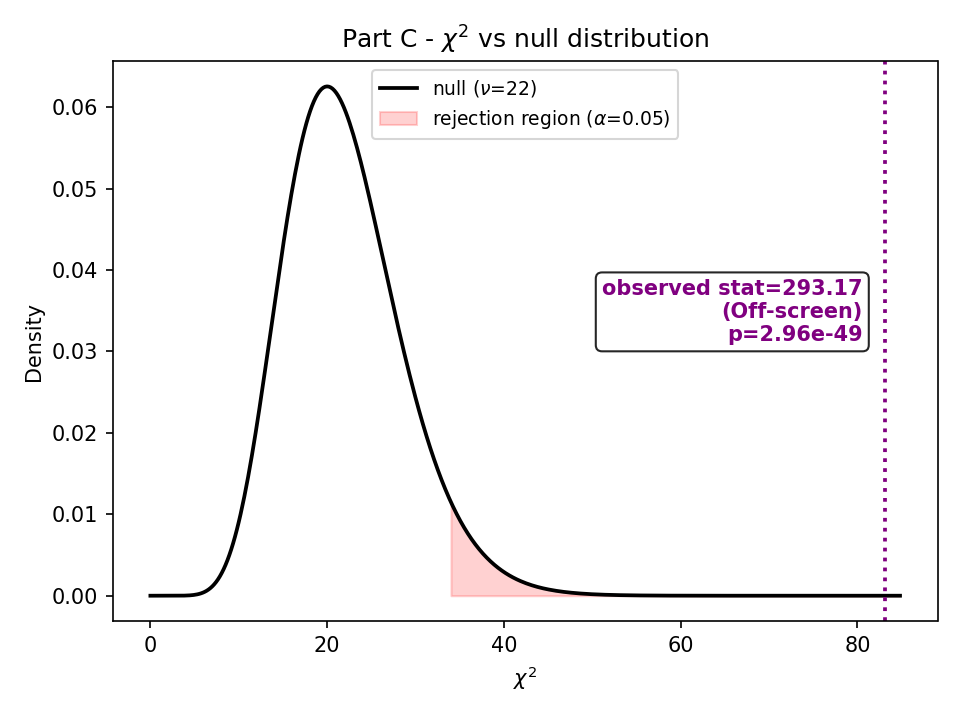
\includegraphics[width=0.60\textwidth]{fig_C2_chi2.png}
		\caption{Null $\chi^2(\nu)$ density with the observed statistic from Part~C.}
		\label{fig:C2}
	\end{figure}
	
	$H_0$ is rejected. Figure~\ref{fig:C3} (as shown later) shows signed standardised residuals $(O_\ell - E_\ell)/\sqrt{E_\ell}$ per letter, with the top-five contributors highlighted in red. The dashed lines mark $\pm 2$ (per-bin 95\% Poisson bands for a single test). 
	
	With $K = 26$ bins, however, the Bonferroni-corrected threshold is $\pm z_{\alpha/2K} = \pm z_{0.05/52} \approx \pm 3.29$: individual letters are only flagged as significant after multiple-comparison correction if $|r| > 3.29$. Several letters (A, M, N, R, L) comfortably exceed this threshold, confirming that the rejection of $H_0$ is not an artefact of multiple comparisons. The distributional shift reflects the alphabetic issuance order: old and new formats cover distinct ranges of the alphabet.
	This is of course due to issues being done in a yearly basis, and old characters running out.
	\begin{figure}[H]
		\centering
		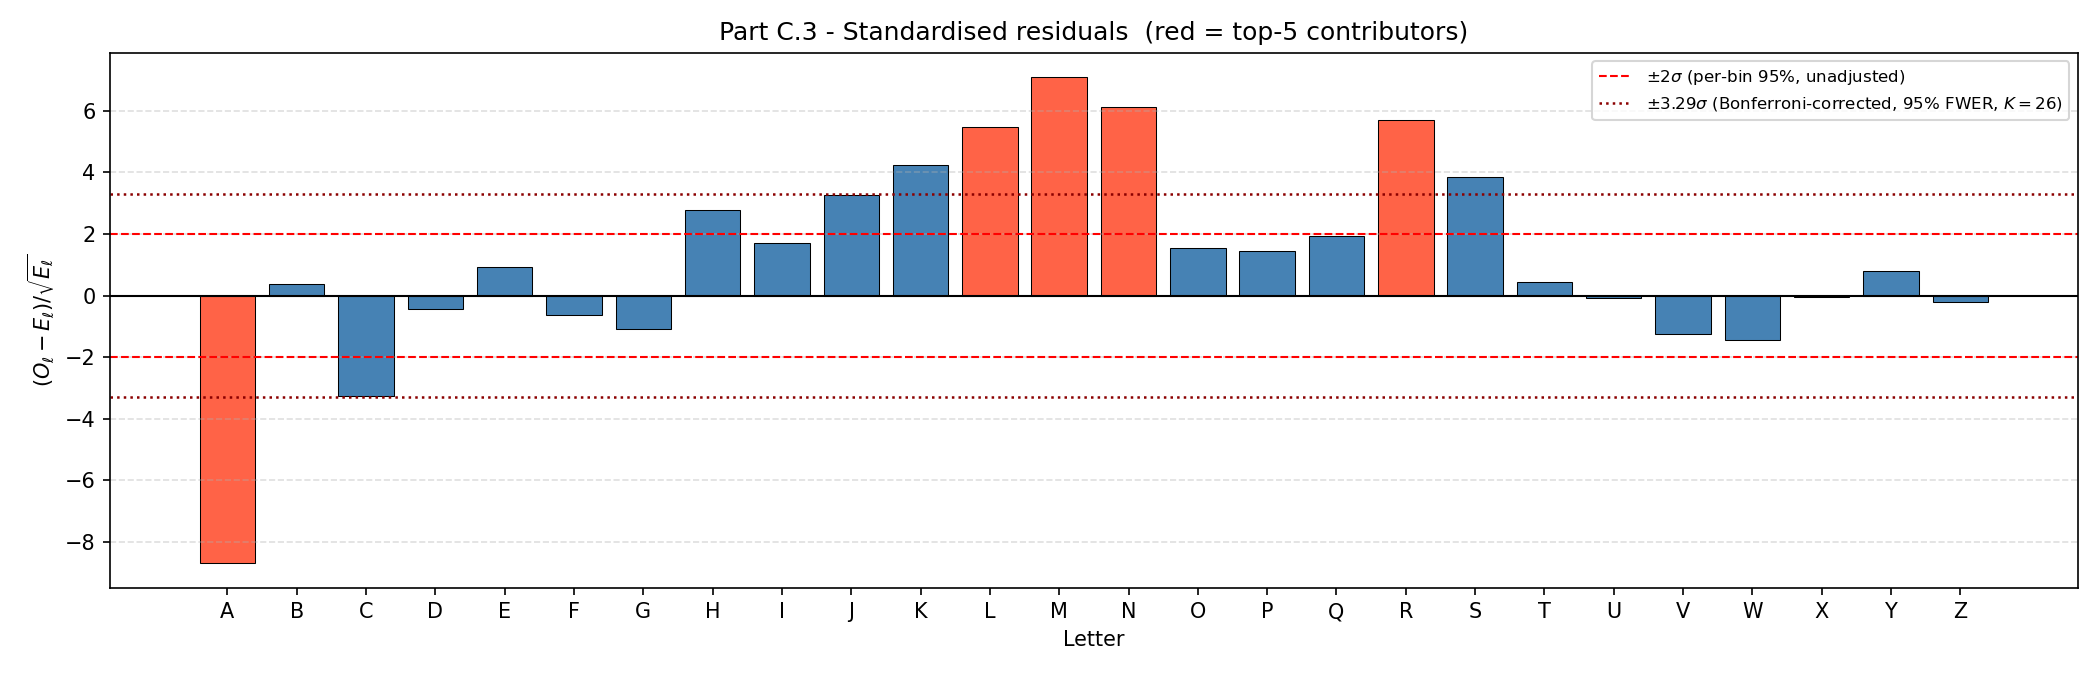
\includegraphics[width=0.90\textwidth]{fig_C3_residuals.png}
		\caption{Standardised residuals per letter. Dashed red lines mark the unadjusted $\pm 2\sigma$ per-bin band; dotted dark red lines mark the Bonferroni-corrected $\pm 3.29\sigma$ threshold (95\% FWER, $K=26$). Red bars are the five largest contributors to $\chi^2$. Note that this is something new I tried to do, references are on the bottom.}
		\label{fig:C3}
	\end{figure}
	
	\section{Part D: Are Certain Letter Pairs Suppressed?}
	
	$H_0$: consecutive letters are drawn independently, so $P(j,k) = \hat{p}_j \cdot \hat{p}_k$ and $E_{jk} = N \hat{p}_j \hat{p}_k$. Each old plate contributes 2 pairs (AB, BC); each new plate contributes 3 (AB, BC, CD). The test is restricted to $K$ letters with $\geq 10$ individual occurrences, ensuring $E_{jk} \geq 5$ throughout; $\nu = K^2 - 1$.
	
	\begin{figure}[H]
		\centering
		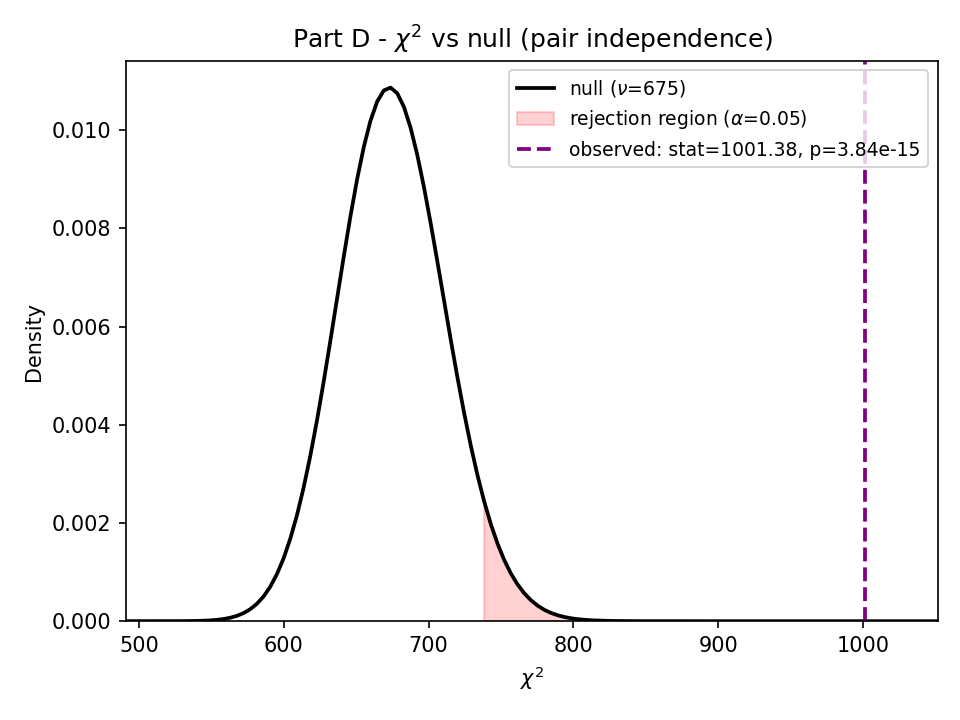
\includegraphics[width=0.60\textwidth]{fig_D1_chi2.png}
		\caption{Null $\chi^2(K^2-1)$ density rescaled to $\pm 5\sigma$ around the null mean due to a suggestion by the professor, with the observed statistic from Part~D marked. The null is centred at $\nu \approx 675$; the observed statistic at $\approx 1001$ falls far into the rejection region ($p = 3.84 \times 10^{-15}$).}
		\label{fig:D1}
	\end{figure}
	
	$H_0$ is strongly rejected. Figure~\ref{fig:D2} shows the full $K \times K$ standardised residual matrix; the five most over- and under-represented pairs are outlined in black. Under-represented pairs are not as apparent for profane words, maybe the dataset is not big enough yet.
	
	\begin{figure}[H]
		\centering
		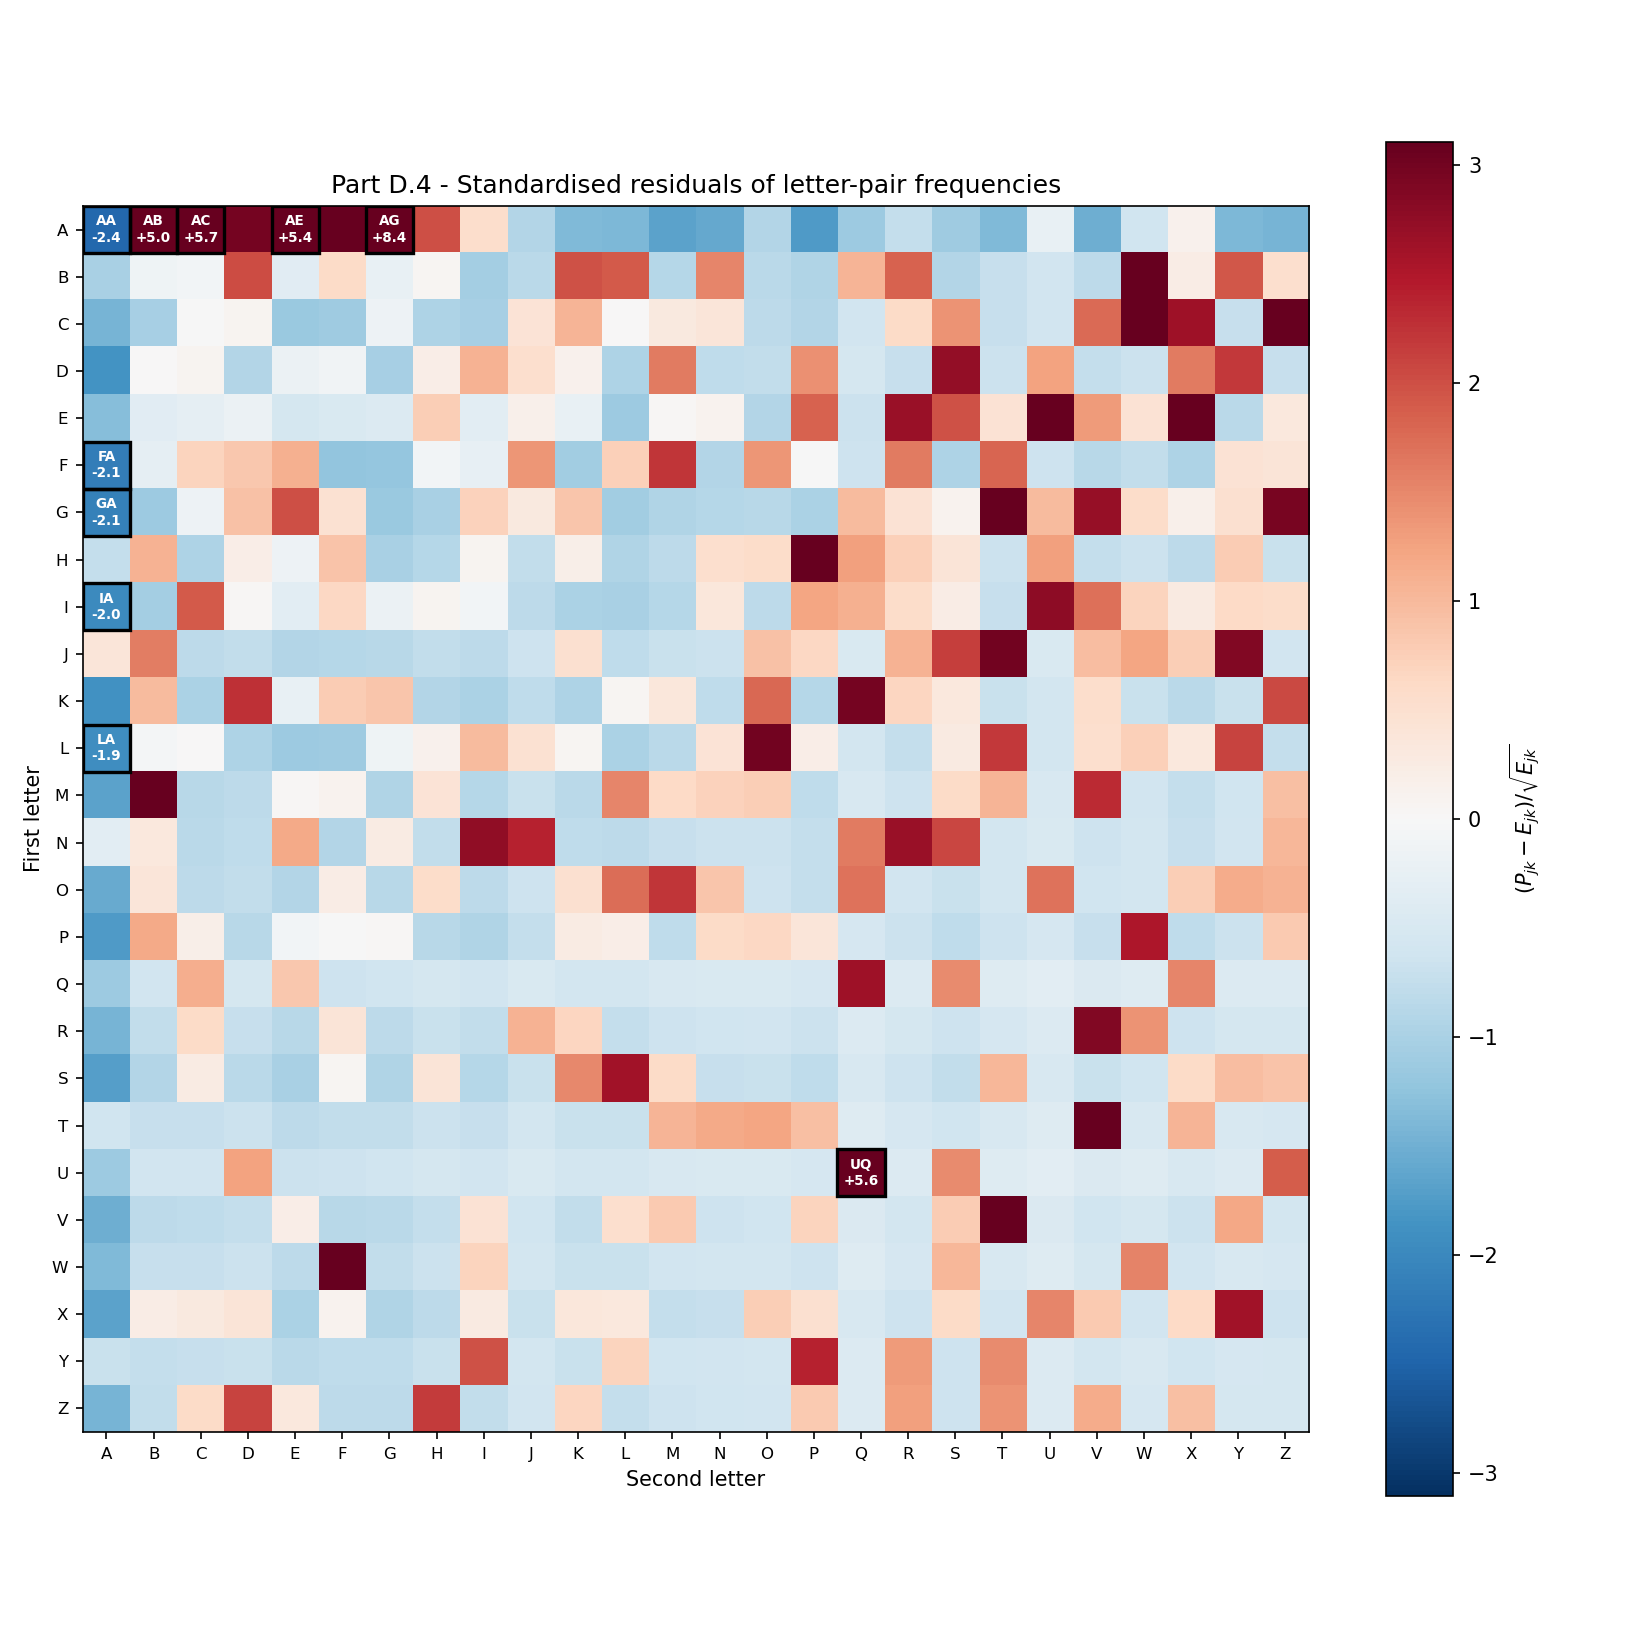
\includegraphics[width=0.90\textwidth]{fig_D2_heatmap.png}
		\caption{Standardised residual matrix $(P_{jk}-E_{jk})/\sqrt{E_{jk}}$. Blue = under-represented; red = over-represented. Black outlines mark the five most extreme pairs in each direction.}
		\label{fig:D2}
	\end{figure}
	
	\section{Part E: Is Our Sample Biased Toward Older or Newer Plates?}
	
	Each plate's registration year is estimated by mapping its alphanumeric code to a known issuance milestone via linear interpolation, using anchor data from Wikipedia's Argentine license plate article.
	
	\subsection*{My Null Hypothesis}
	$H_0$: the mean estimated year equals the midpoint of the full Argentine issuance range. If our 219 plates were a uniform random draw from every plate ever issued, the expected mean would be
	\[
	\mu_0 = \frac{\text{earliest anchor} + \text{collection year}}{2} = \frac{1995 + 2026}{2} = 2010.5.
	\]
	A significant result indicates that the street sample is temporally skewed: $t > 0$ means over-representation of newer plates; $t < 0$ means older plates dominate.
	
	\subsection*{My Results}
	We apply a one-sample $t$-test with $\nu = n - 1$ degrees of freedom and report the 95\% CI on the mean.
	
	\begin{figure}[H]
		\centering
		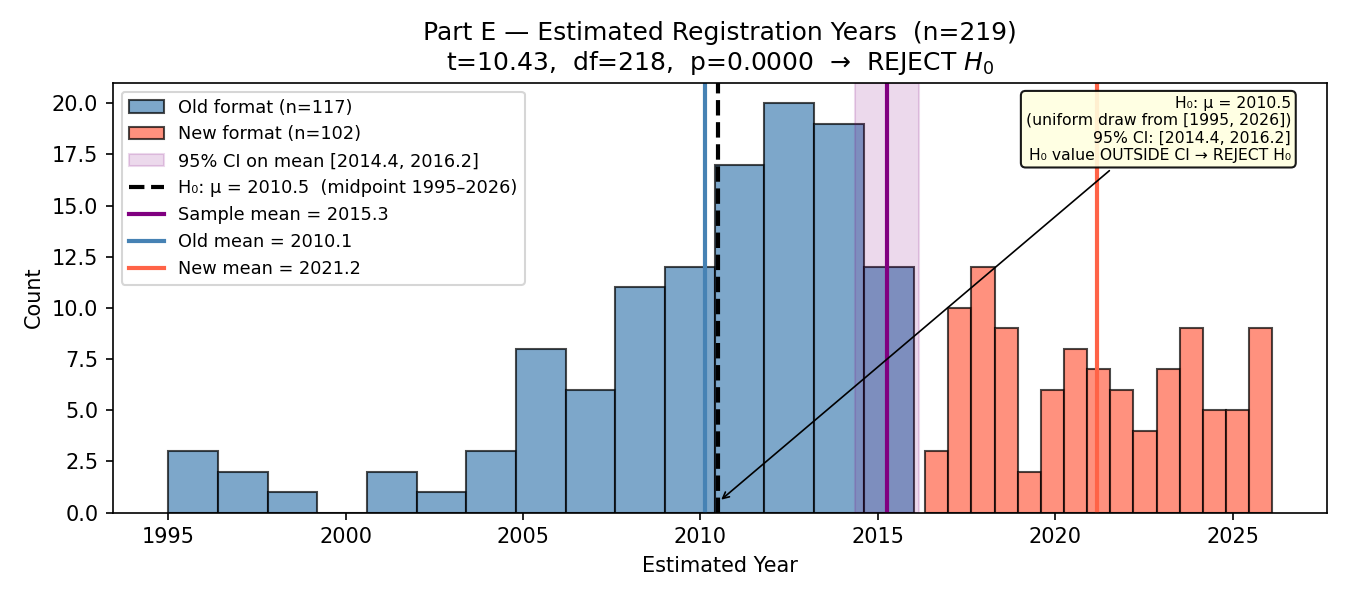
\includegraphics[width=0.85\textwidth]{fig_E1_years.png}
		\caption{Estimated registration years for old-format (blue) and new-format (red) plates. The dashed black line is $H_0: \mu_0 = 2010.5$ (midpoint 1995-2026); the purple shaded band is the 95\% CI on the sample mean. If the dashed line falls outside the band, $H_0$ is rejected. Annotations boxes were a nightmare.}
		\label{fig:E1}
	\end{figure}
	
	\begin{figure}[H]
		\centering
		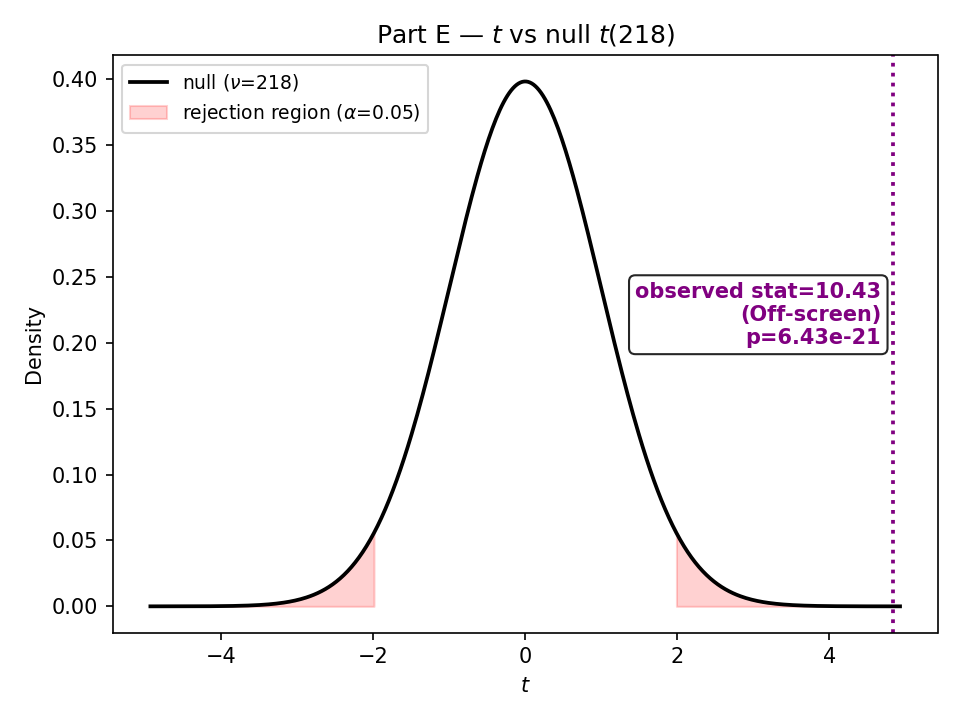
\includegraphics[width=0.60\textwidth]{fig_E2_ttest.png}
		\caption{Null $t(\nu)$ density (two-tailed) with the observed $t$-statistic for Part~E.}
		\label{fig:E2}
	\end{figure}
	
	If $H_0$ is rejected and $t > 0$, the sample skews toward newer vehicles an expected result for a street convenience sample, where recently registered cars are more common.
	
	\section*{Conclusion}
	Digit frequencies are consistent with a uniform distribution and mean digit sums do not differ between formats (Parts A--B), suggesting no detectable administrative pattern in digit assignment. Letter distributions differ significantly between formats (Part~C), reflecting their distinct alphabetic issuance ranges; several letters remain significant even after Bonferroni correction. Consecutive letter pairs deviate strongly from independence (Part~D), sort of consistent with a deliberate suppression policy for certain syllable combinations, more data is needed. Part~E tests whether the street sample is temporally representative of the full plate registry. (See Slides I provided to see the comparison with Argentinian vehicles)
	
\section*{Biographies/Sources.}
\begin{itemize}
	\item Cowan, Glen. \textit{Statistical Data Analysis in Particle Physics}. Oxford University Press, 1998.
	\item SciPy Documentation. \texttt{scipy.stats} module. \texttt{https://docs.scipy.org}
	\item Wikipedia. ``Vehicle registration plates of Argentina.'' \texttt{https://en.wikipedia.org/wiki/Vehicle\_registration\_plates\_of\_Argentina}
	\item Wikipedia. ``Bonferroni correction.'' \texttt{https://en.wikipedia.org/wiki/Bonferroni\_correction}
	\item AI Assistance: Claude (Anthropic). Helped with formatting, \LaTeX\ structuring, and statistical methodology documentation.
	\item Python Graph Gallery. Matplotlib examples. \texttt{https://python-graph-gallery.com}
\end{itemize}
	
\end{document}